\documentclass[../main.tex]{subfiles}

\begin{document}

% ===========================================================================
\subsection{Introducción}
% ===========================================================================

Los sistemas de información sanitaria acumulan, a lo largo de décadas, un volumen de datos que los esquemas de base de datos tradicionales no siempre están en condiciones de gestionar con eficiencia. Un historial médico longitudinal completo no es una entidad estática: crece con cada consulta, cada ingreso, cada prescripción farmacológica y cada baja laboral que el paciente experimenta a lo largo de su vida. La heterogeneidad de ese crecimiento —eventos muy frecuentes mezclados con registros históricos que raramente se vuelven a leer— plantea un problema de optimización que no tiene una respuesta única ni sencilla.

A esa complejidad técnica se le superpone, además, una exigencia legal de primer orden. El Reglamento General de Protección de Datos (RGPD, Reglamento UE 2016/679)~\cite{rgpd2016} establece que los datos de salud pertenecen a la categoría de \textit{datos especialmente protegidos} y que su tratamiento debe cumplir, entre otros principios, el de \textbf{privacidad por diseño y por defecto}. En la práctica, esto significa que la separación entre los datos clínicos y los datos identificativos del paciente no puede ser una capa de seguridad que se añade a posteriori sobre un sistema ya construido: tiene que ser una decisión arquitectónica tomada antes de escribir la primera línea de código.

Partiendo de estas dos premisas —optimización del rendimiento y cumplimiento normativo—, el presente proyecto diseña e implementa \textbf{ChronoHealthDB}, una base de datos de historiales médicos longitudinales que aborda simultáneamente ambas cuestiones. El modelo separa la información clínica de la información identificativa mediante un puente criptográfico basado en el algoritmo SHA-256, de modo que los análisis epidemiológicos pueden operar sobre datos completamente pseudoanonimizados sin que sea necesario acceder en ningún momento a los datos personales del paciente. Al mismo tiempo, se explota la capacidad de MySQL~8 de combinar distintos \textit{storage engines} bajo un mismo servidor, asignando a cada tabla el motor más adecuado según su patrón de acceso específico.

Los tres objetivos que articulan el trabajo son los siguientes:

\begin{enumerate}
    \item Diseñar un modelo relacional que implemente la separación de datos personales y clínicos conforme al principio de privacidad por diseño del RGPD, haciendo inviable el acceso accidental a información identificativa desde el modelo epidemiológico.
    \item Optimizar el rendimiento del sistema mediante una arquitectura multi-motor que asigne a cada tabla el \textit{storage engine} más apropiado para su patrón concreto de escritura, lectura y archivado.
    \item Validar empíricamente, mediante una batería de benchmarks controlados, el impacto de los índices y de la elección de motor sobre el tiempo de respuesta y el espacio de almacenamiento.
\end{enumerate}

% ===========================================================================
\subsection{Tecnologías Empleadas en la Fase Relacional}
% ===========================================================================

\subsubsection*{MySQL 8.0}

La elección de MySQL 8.0 como sistema gestor de base de datos principal responde a una característica que, a efectos de este proyecto, resulta decisiva: la posibilidad de mezclar múltiples \textit{storage engines} bajo un mismo servidor e incluso dentro de una misma base de datos. En entornos de producción homogéneos, todas las tablas suelen utilizar el mismo motor por comodidad operativa. Sin embargo, cuando los requisitos de distintas tablas son tan dispares como los de un historial longitudinal activo, un archivo histórico inmutable y una cola de trabajo en tiempo real, la capacidad de especializar cada tabla por separado se convierte en una ventaja real y, como veremos, medible.

A ello se añade que MySQL 8.0 introduce mejoras sustanciales respecto a versiones anteriores: soporte nativo de expresiones de tabla común (CTE) y funciones de ventana, mejoras en el optimizador de consultas con histogramas de columna, y un motor InnoDB revisado con mejor gestión del \textit{buffer pool}. Para los propósitos del benchmarking que se describe más adelante, disponer de un optimizador de consultas maduro es esencial para obtener resultados representativos.

\subsubsection*{Arquitectura multi-motor}

El núcleo técnico del proyecto es la asignación de un motor distinto a cada tabla en función de su rol en el sistema. La Tabla~\ref{tab:motores} resume esta decisión de diseño.

\begin{table}[htbp]
    \centering
    \caption{Asignación de motor de almacenamiento por tipo de tabla en ChronoHealthDB.}
    \label{tab:motores}
    \small
    \begin{tabular}{lllp{5.2cm}}
        \toprule
        \textbf{Tabla} & \textbf{Motor} & \textbf{Patrón de acceso} & \textbf{Justificación principal} \\
        \midrule
        \texttt{paciente\_anonimo}         & InnoDB  & Lectura/escritura continua    & ACID, claves foráneas, MVCC \\
        \texttt{datos\_personales}         & InnoDB  & Lectura/escritura controlada  & Integridad transaccional y referencial \\
        \texttt{evento\_clinico}           & InnoDB  & Inserción + consulta intensiva & Índices compuestos, soporte de FK \\
        \texttt{historico\_bajas\_medicas} & ARCHIVE & Solo INSERT + SELECT masivo   & Compresión automática \textit{zlib} \\
        \texttt{triaje\_urgencias\_actual} & MEMORY  & Cola en RAM, alta frecuencia  & Latencia sub-milisegundo \\
        \bottomrule
    \end{tabular}
\end{table}

\textbf{InnoDB}~\cite{mysql8innodb} es el motor transaccional por defecto de MySQL 8 y el más completo en cuanto a funcionalidades. Implementa transacciones ACID completas, bloqueo a nivel de fila y \textit{Multi-Version Concurrency Control} (MVCC), que permite lecturas consistentes sin bloquear las escrituras concurrentes. Es el motor apropiado para toda la información que debe modificarse, relacionarse con otras tablas mediante claves foráneas o participar en transacciones reversibles.

\textbf{ARCHIVE}~\cite{mysql8archive} es un motor diseñado específicamente para el almacenamiento de grandes volúmenes de datos históricos inmutables. Aplica compresión \textit{zlib}~\cite{rfc1950zlib} fila a fila en el momento de la inserción, lo que reduce el espacio en disco de forma drástica. A cambio, no soporta claves foráneas, no permite operaciones UPDATE ni DELETE, y sus capacidades de indexación son mínimas. Para un historial de bajas médicas que, por imperativo normativo, debe conservarse intacto una vez emitido, estas restricciones no constituyen un problema operativo.

\textbf{MEMORY}~\cite{mysql8memory} (anteriormente denominado HEAP) almacena sus datos íntegramente en la memoria RAM del servidor. La ausencia de operaciones de E/S a disco se traduce en latencias de acceso significativamente menores que las de cualquier motor basado en almacenamiento persistente. Sus limitaciones —pérdida de datos al reiniciar el servidor, sin soporte de claves foráneas ni transacciones complejas— lo hacen inadecuado para datos permanentes, pero es la opción óptima para colas temporales de alta frecuencia como el registro de pacientes activos en urgencias.

\subsubsection*{Python, Faker y PyMySQL}

La generación de un volumen de datos lo suficientemente grande como para que los benchmarks sean estadísticamente representativos requería una herramienta de automatización. Se utilizó Python~3.12 con la biblioteca \texttt{Faker} (localización \texttt{es\_ES}) para sintetizar datos personales coherentes con la realidad española: nombres, apellidos y NIF válidos, números de la Seguridad Social de doce dígitos, provincias y municipios reales. El conector \texttt{PyMySQL} se empleó para las operaciones de inserción masiva contra el servidor MySQL.

Lo que hace distinto a este generador es su \textbf{combinatoria clínica}: en lugar de insertar cadenas de texto aleatorias en los campos de descripción médica, el script construye frases plausibles combinando fragmentos predefinidos de estado general del paciente, hallazgos de exploración física, factores de riesgo y notas clínicas. El resultado es un conjunto de datos que, a efectos de consulta y análisis, se comporta como datos reales procedentes de un entorno de producción.

% ===========================================================================
\subsection{Desarrollo del Proyecto con MySQL}
% ===========================================================================

\subsubsection{Diseño del Modelo Relacional}

Antes de entrar en los detalles, conviene tener una visión de conjunto del modelo. La base de datos se articula en torno a cinco tablas, cada una con un papel bien definido dentro del flujo de trabajo sanitario. El diagrama EER (\textit{Enhanced Entity-Relationship}) de la Figura~\ref{fig:eer} muestra la estructura completa tal y como la diseñamos en MySQL Workbench, con sus columnas, tipos de datos y las relaciones que las conectan.

El paciente se representa de forma desdoblada: \texttt{paciente\_anonimo} guarda toda la información clínica y demográfica sin nada que identifique a la persona, mientras que \texttt{datos\_personales} contiene el nombre, el DNI y el número de la Seguridad Social. Ambas tablas se unen mediante una relación identificadora 1:1. De \texttt{paciente\_anonimo} cuelga \texttt{evento\_clinico} con una relación 1:N, que es donde se acumula el historial longitudinal (cada paciente tiene varios eventos a lo largo del tiempo). Por último, \texttt{historico\_bajas\_medicas} y \texttt{triaje\_urgencias\_actual} se vinculan al paciente a través del \texttt{codigo\_hash}, sin clave foránea declarada, por los motivos que se explican más adelante.

\begin{figure}[htbp]
    \centering
    
\includegraphics[width=\textwidth]{nuestra_base_de_datos.jpg}
    \caption{Diagrama EER completo de ChronoHealthDB en MySQL Workbench. Se aprecian las cinco tablas del sistema y sus relaciones: la separación 1:1 entre \texttt{paciente\_anonimo} y \texttt{datos\_personales}, la relación 1:N hacia \texttt{evento\_clinico} y las dos tablas auxiliares (\texttt{historico\_bajas\_medicas} y \texttt{triaje\_urgencias\_actual}) enlazadas por el \texttt{codigo\_hash}.}
    \label{fig:eer}
\end{figure}

La base de datos se crea con el juego de caracteres \texttt{utf8mb4} y la colación \texttt{utf8mb4\_unicode\_ci}. La elección de \texttt{utf8mb4} sobre la variante \texttt{utf8} de MySQL es deliberada: la implementación interna de \texttt{utf8} en MySQL es una variante reducida a tres bytes por carácter que excluye el plano suplementario Unicode, con lo que cualquier carácter fuera del BMP —emojis, caracteres de escrituras asiáticas modernas— provocaría errores silenciosos de truncado. \texttt{utf8mb4} es la implementación correcta del estándar y debe ser la elección predeterminada en cualquier sistema que no pueda garantizar la homogeneidad del conjunto de caracteres introducido por los usuarios.

\paragraph{El puente criptográfico: hash SHA-256}

El elemento arquitectónico central del modelo es la separación entre \texttt{paciente\_anonimo} y \texttt{datos\_personales}. Ambas tablas comparten la misma clave primaria numérica (\texttt{id\_paciente}) y el mismo valor de \texttt{codigo\_hash}, pero sirven propósitos radicalmente distintos.

El campo \texttt{codigo\_hash} se obtiene aplicando el algoritmo SHA-256~\cite{fips180sha256} al número del documento de identidad del paciente (véase el Listado~\ref{lst:sha256}). El resultado es una cadena hexadecimal de 64 caracteres (256 bits) que actúa como huella digital determinista del individuo sin revelar su identidad. Un investigador que opere exclusivamente sobre \texttt{paciente\_anonimo} puede agregar todos los eventos clínicos de un mismo individuo a través de \texttt{codigo\_hash} sin tener en ningún momento acceso al DNI o al nombre real del paciente.

\begin{lstlisting}[language=Python, caption={Generación del identificador anónimo mediante SHA-256 del documento de identidad.}, label={lst:sha256}]
import hashlib

# El NIF del paciente nunca se almacena en el modelo anonimo
codigo_hash = hashlib.sha256(
    documento_identidad.encode()
).hexdigest()  # Cadena hexadecimal de 64 caracteres
\end{lstlisting}

\paragraph{Relación identificadora 1:1 con \texttt{ON DELETE RESTRICT}}

La relación entre \texttt{paciente\_anonimo} y \texttt{datos\_personales} es una relación identificadora uno a uno: la clave primaria de \texttt{datos\_personales} es simultáneamente su clave foránea, lo que en el modelo relacional se denomina \textit{identifying relationship}. La cláusula \texttt{ON DELETE RESTRICT} impide eliminar un registro del modelo anónimo mientras exista su correspondiente ficha en el modelo personal, evitando así huérfanos referenciales. El Listado~\ref{lst:tablas_core} muestra la definición de ambas tablas.

\begin{lstlisting}[language=SQL, caption={Tablas \texttt{paciente\_anonimo} y \texttt{datos\_personales}: relación identificadora 1:1 con integridad referencial.}, label={lst:tablas_core}]
CREATE TABLE IF NOT EXISTS paciente_anonimo (
    id_paciente          INT UNSIGNED  NOT NULL AUTO_INCREMENT,
    codigo_hash          CHAR(64)      NOT NULL,
    anio_nacimiento      YEAR          NOT NULL,
    sexo_biologico       ENUM('M','F','Indeterminado') NOT NULL,
    grupo_sanguineo      ENUM('A+','A-','B+','B-','AB+',
                              'AB-','O+','O-','Desconocido') NOT NULL,
    region_sanitaria     VARCHAR(100)  NOT NULL,
    factores_riesgo      TEXT          NULL,
    activo               TINYINT(1)    NOT NULL DEFAULT 1,
    PRIMARY KEY (id_paciente),
    UNIQUE KEY uq_codigo_hash (codigo_hash),
    INDEX idx_sexo_anio (sexo_biologico, anio_nacimiento),
    INDEX idx_activo    (activo)
) ENGINE=InnoDB DEFAULT CHARSET=utf8mb4 COLLATE=utf8mb4_unicode_ci;

CREATE TABLE IF NOT EXISTS datos_personales (
    id_paciente          INT UNSIGNED  NOT NULL,
    codigo_hash          CHAR(64)      NOT NULL,
    nombre               VARCHAR(100)  NOT NULL,
    primer_apellido      VARCHAR(100)  NOT NULL,
    documento_identidad  VARCHAR(20)   NOT NULL,
    num_seguridad_social VARCHAR(30)   NOT NULL,
    consentimiento_rgpd  TINYINT(1)   NOT NULL DEFAULT 0,
    PRIMARY KEY (id_paciente),
    UNIQUE KEY uq_documento  (documento_identidad),
    UNIQUE KEY uq_nss        (num_seguridad_social),
    CONSTRAINT fk_dp_paciente FOREIGN KEY (id_paciente)
        REFERENCES paciente_anonimo (id_paciente)
        ON DELETE RESTRICT ON UPDATE CASCADE
) ENGINE=InnoDB DEFAULT CHARSET=utf8mb4 COLLATE=utf8mb4_unicode_ci;
\end{lstlisting}

La tabla \texttt{historico\_bajas\_medicas} referencia al paciente mediante su \texttt{codigo\_hash} como columna de texto ordinaria, sin declarar clave foránea. Esta solución de compromiso es una consecuencia directa de la limitación del motor ARCHIVE, que no admite restricciones referenciales. Se acepta conscientemente a cambio de los beneficios de compresión que se analizan en el apartado~\ref{sec:benchmark_espacial}.

\paragraph{Enfoque OLTP y ausencia de una dimensión Tiempo explícita}

Una pregunta que nos surgió durante el diseño fue si convenía modelar el tiempo como una dimensión propia, al estilo de un esquema en estrella de un \textit{data warehouse}, con una tabla \texttt{tiempo} a la que apuntaran las claves foráneas de los eventos. Tras valorarlo, decidimos no hacerlo, y creemos que la decisión está justificada. Añadir una tabla física explícita denominada \texttt{tiempo} requeriría rediseñar el diagrama EER, modificar las claves foráneas, reescribir el generador de datos en Python para insertar los registros dimensionales y reestructurar todas las consultas SQL y XML realizadas hasta ahora. A nivel de ingeniería, en un sistema que gestiona colas en tiempo real (triaje) y registros clínicos longitudinales, el diseño OLTP actual es preciso y evita la sobrecarga de uniones (JOIN) innecesarias para consultar una fecha. En otras palabras, las dimensiones temporales (año, mes, día) son tan baratas de calcular sobre las propias columnas \texttt{DATE} mediante funciones nativas de MySQL como \texttt{YEAR()} o \texttt{MONTH()} que el coste de mantener una tabla de calendario separada no compensaría: estaríamos pagando complejidad y JOINs adicionales para resolver algo que el motor ya hace de forma directa. Un esquema en estrella tiene todo el sentido cuando el objetivo principal es la explotación analítica masiva (OLAP); aquí, en cambio, el patrón de uso dominante es transaccional —dar de alta a un paciente en triaje, abrir su ficha, registrar un evento—, y para eso el modelo normalizado orientado a transacciones es la opción correcta.

% ---------------------------------------------------------------------------
\subsubsection{Seguridad y Gestión de Roles}
% ---------------------------------------------------------------------------

La política de seguridad del sistema se basa en el principio de \textbf{mínimo privilegio}: cada cuenta de usuario de la base de datos recibe exactamente los permisos que necesita para cumplir su función y ninguno más. Se definen dos perfiles con responsabilidades complementarias y claramente diferenciadas.

El usuario \texttt{doctor} modela una aplicación clínica (HIS). Puede consultar e insertar datos en todas las tablas del sistema, incluyendo \texttt{datos\_personales}, y dispone de permiso de eliminación sobre \texttt{triaje\_urgencias\_actual} para poder dar el alta a los pacientes que abandonan urgencias. En cambio, carece de permisos de borrado sobre el historial clínico longitudinal: un evento registrado en \texttt{evento\_clinico} no puede eliminarse de la base de datos, lo que garantiza la integridad del historial a largo plazo.

El usuario \texttt{investigador} tiene acceso de solo lectura (\texttt{SELECT}) y únicamente sobre las tablas sin datos personales identificativos: \texttt{paciente\_anonimo}, \texttt{evento\_clinico} e \texttt{historico\_bajas\_medicas}. La tabla \texttt{datos\_personales} le está completamente vetada, lo que garantiza que cualquier análisis epidemiológico opere exclusivamente sobre información pseudoanonimizada.

\begin{lstlisting}[language=SQL, caption={Creación de usuarios y asignación de privilegios mínimos.}, label={lst:usuarios}]
-- Cuenta de aplicacion clinica
CREATE USER IF NOT EXISTS 'doctor'@'%'
    IDENTIFIED BY 'Medicina_2026*';

GRANT SELECT, INSERT, UPDATE
    ON PROYECTO.paciente_anonimo       TO 'doctor'@'%';
GRANT SELECT, INSERT, UPDATE
    ON PROYECTO.datos_personales       TO 'doctor'@'%';
GRANT SELECT, INSERT, UPDATE
    ON PROYECTO.evento_clinico         TO 'doctor'@'%';
GRANT SELECT, INSERT, UPDATE, DELETE
    ON PROYECTO.triaje_urgencias_actual TO 'doctor'@'%';
GRANT SELECT, INSERT
    ON PROYECTO.historico_bajas_medicas TO 'doctor'@'%';

-- Cuenta de investigacion (solo tablas anonimizadas, solo lectura)
CREATE USER IF NOT EXISTS 'investigador'@'%'
    IDENTIFIED BY 'Bioinfo_2026*';

GRANT SELECT ON PROYECTO.paciente_anonimo        TO 'investigador'@'%';
GRANT SELECT ON PROYECTO.evento_clinico          TO 'investigador'@'%';
GRANT SELECT ON PROYECTO.historico_bajas_medicas TO 'investigador'@'%';

FLUSH PRIVILEGES;
\end{lstlisting}

Resulta especialmente significativo lo que el usuario \texttt{investigador} \textit{no puede hacer}: no tiene acceso a \texttt{datos\_personales} ni a \texttt{triaje\_urgencias\_actual}. Esta restricción no está implementada a nivel de aplicación, donde podría ser fácilmente eludida; está implementada directamente en el motor de base de datos, con lo que ningún código que use esa cuenta podrá acceder a esa información aunque lo intente.

La Figura~\ref{fig:roles} muestra el panel de gestión de usuarios de MySQL Workbench confirmando la creación correcta de ambas cuentas.

\begin{figure}[htbp]
    \centering
    
\includegraphics[width=0.5\textwidth]{roles_doctor_investigador.jpg}
    \caption{Panel \textit{Users and Privileges} de MySQL Workbench. Los usuarios \texttt{doctor} e \texttt{investigador} aparecen correctamente creados con alcance global (\texttt{\%}).}
    \label{fig:roles}
\end{figure}

% ---------------------------------------------------------------------------
\subsubsection{Población Sintética de Datos}
% ---------------------------------------------------------------------------

Para que los benchmarks sean representativos de un entorno de producción, se necesita un volumen de datos suficientemente grande. El script \texttt{generador\_datos.py} utiliza \texttt{Faker~(es\_ES)} para generar datos personales coherentes con la realidad española y construye cada registro siguiendo una lógica de combinatoria clínica: las descripciones de eventos, los factores de riesgo y las notas clínicas se obtienen combinando fragmentos predefinidos de texto médico plausible, de modo que el resultado tiene coherencia semántica y no produce cadenas sin sentido que distorsionarían los patrones de consulta.

Cada paciente sintético generado tiene entre 2 y 6 eventos clínicos distribuidos a lo largo de los últimos cinco años, el 15\% tiene al menos un registro en el histórico de bajas médicas, y el 2\% está presente en la cola activa de triaje de urgencias. Al concluir la ejecución completa del generador, la base de datos contiene \textbf{40.000 historiales clínicos} (Figura~\ref{fig:recuento}), lo que da lugar a una tabla \texttt{evento\_clinico} con aproximadamente 160.000--180.000 filas: un volumen más que suficiente para que las diferencias de rendimiento entre estrategias de acceso sean claramente perceptibles.

\begin{figure}[htbp]
    \centering
    
\includegraphics[width=0.85\textwidth]{recuento_pacientes_insertados.jpg}
    \caption{Terminal de PowerShell mostrando la finalización del proceso de generación masiva de datos: 40.000 historiales clínicos insertados correctamente en la base de datos.}
    \label{fig:recuento}
\end{figure}

% ---------------------------------------------------------------------------
\subsubsection{Optimización Temporal: Benchmarking de Consultas}
\label{sec:benchmark_temporal}
% ---------------------------------------------------------------------------

Se diseñaron tres consultas representativas de los patrones de acceso más habituales en un sistema sanitario. Para cada una se midió el tiempo de ejecución en dos escenarios: sin índice auxiliar y con el índice correspondiente activo. Adicionalmente, las consultas 1 y 3 se evaluaron en motores alternativos (MyISAM y MEMORY, respectivamente) para cuantificar el efecto de la selección del motor más allá de la indexación.

Todas las mediciones de tiempo se obtienen como la \textbf{media aritmética de 50 ejecuciones consecutivas} con el script \texttt{medidor\_tiempos.py}, lo que reduce la influencia de la variabilidad de caché, gestión de memoria y carga del sistema operativo. Las estadísticas de coste estimado proceden del \textit{Visual Explain} de MySQL Workbench.

% ---- CONSULTA 1 ------------------------------------------------
\paragraph{Consulta 1: agregación temporal con filtro de rango de fechas}

La primera consulta cuenta el número de eventos clínicos registrados durante un mes concreto:

\begin{lstlisting}[language=SQL, caption={Consulta 1: conteo de eventos en un rango temporal de un mes.}, label={lst:q1}]
SELECT COUNT(*) AS total_eventos
FROM   evento_clinico
WHERE  fecha_evento BETWEEN '2023-01-01' AND '2023-01-31';
\end{lstlisting}

Esta operación es representativa de los informes estadísticos mensuales que cualquier sistema sanitario genera de forma rutinaria. Sin un índice sobre la columna \texttt{fecha\_evento}, el optimizador no dispone de ninguna estructura de acceso directo y debe leer la totalidad de las filas de la tabla. El \textit{Visual Explain} (Figura~\ref{fig:q1_sin_indice}) lo confirma: el plan de ejecución muestra un \textbf{Full Table Scan} marcado en rojo, con un coste estimado de $19.543{,}10$ y 183.010 filas inspeccionadas. Las \textit{Query Statistics} de Workbench (Figura~\ref{fig:q1_stats_sin}) registran un tiempo de ejecución en servidor de $60{,}9$~ms.

\begin{figure}[htbp]
    \centering
    \begin{subfigure}[b]{0.48\textwidth}
        \centering
        
\includegraphics[width=\textwidth]{consulta1_sin_indice.png}
        \caption{\textit{Full Table Scan} (rojo). Coste: 19.543,10. Filas inspeccionadas: 183.010.}
        \label{fig:q1_sin_indice}
    \end{subfigure}
    \hfill
    \begin{subfigure}[b]{0.48\textwidth}
        \centering
        
\includegraphics[width=\textwidth]{consulta1_con_indice.jpg}
        \caption{\textit{Index Range Scan} (ámbar). Coste: 643,62. Filas: 3.210.}
        \label{fig:q1_con_indice}
    \end{subfigure}
    \caption{\textit{Visual Explain} de la Consulta~1 sin índice (izquierda) y con el índice \texttt{idx\_fecha\_evento} activo (derecha). La diferencia de coste estimado es de un factor 30,4×.}
    \label{fig:q1_explain}
\end{figure}

\begin{figure}[htbp]
    \centering
    \begin{subfigure}[b]{0.48\textwidth}
        \centering
        
\includegraphics[width=\textwidth]{tiempo_consulta1_sin_indice.jpg}
        \caption{Sin índice: tiempo servidor 60,9~ms. \textit{Full table scan}: 1.}
        \label{fig:q1_stats_sin}
    \end{subfigure}
    \hfill
    \begin{subfigure}[b]{0.48\textwidth}
        \centering
        
\includegraphics[width=\textwidth]{tiempo_consulta1_con_indice.jpg}
        \caption{Con índice: tiempo servidor 1,1~ms. \textit{Full table scan}: 0. \textit{Select\_range}: 1.}
        \label{fig:q1_stats_con}
    \end{subfigure}
    \caption{\textit{Query Statistics} de Workbench para la Consulta~1. La presencia del índice elimina completamente el escaneo de tabla.}
    \label{fig:q1_stats}
\end{figure}

Tras definir el índice \texttt{idx\_fecha\_evento} sobre \texttt{fecha\_evento}, el comportamiento cambia radicalmente. El plan de ejecución pasa a un \textbf{Index Range Scan} con coste $643{,}62$ y solo 3.210 filas inspeccionadas (Figura~\ref{fig:q1_con_indice}): el optimizador ya no recorre toda la tabla, sino que navega directamente por el árbol B+ hasta el rango correspondiente a enero. Las \textit{Query Statistics} (Figura~\ref{fig:q1_stats_con}) registran un tiempo servidor de $1{,}1$~ms.

La medición estadística a través del script Python (Figura~\ref{fig:q1_python}) confirma la diferencia sobre 50 ejecuciones: el tiempo medio pasa de $46{,}06$~ms sin índice a $1{,}36$~ms con índice, una \textbf{aceleración de 33,8×}.

\begin{figure}[htbp]
    \centering
    
\includegraphics[width=0.88\textwidth]{consulta1_tiempos_python.jpg}
    \caption{Salida del script \texttt{medidor\_tiempos.py} para la Consulta~1: 46,06~ms sin índice (primera ejecución) y 1,36~ms con índice (segunda ejecución), ambas medias de 50 iteraciones.}
    \label{fig:q1_python}
\end{figure}

Adicionalmente, se comparó el motor InnoDB con MyISAM sobre la misma consulta con índice activo. Dado que MyISAM no admite claves foráneas, fue necesario clonar la tabla \texttt{evento\_clinico} sin restricciones referenciales para poder asignarle el motor alternativo. La Figura~\ref{fig:q1_motores} muestra los resultados: InnoDB obtiene $1{,}40$~ms y MyISAM alcanza $1{,}20$~ms, un $14{,}3\%$ menos. La ventaja de MyISAM se explica por la ausencia de la gestión MVCC y del \textit{undo log} transaccional, que reducen la sobrecarga por operación a costa de renunciar a las garantías ACID.

\begin{figure}[htbp]
    \centering
    
\includegraphics[width=0.88\textwidth]{consulta1_motores_InnoDB_vs_MyISAM.jpg}
    \caption{Comparativa InnoDB (1,40~ms) vs.\ MyISAM (1,20~ms) en la Consulta~1 con índice activo (50 iteraciones). MyISAM es más rápido en lecturas puras por carecer de sobrecarga transaccional.}
    \label{fig:q1_motores}
\end{figure}

% ---- CONSULTA 2 ------------------------------------------------
\paragraph{Consulta 2: JOIN entre paciente anónimo y evento clínico}

La segunda consulta recupera el historial completo de un paciente concreto cruzando las dos tablas principales del sistema:

\begin{lstlisting}[language=SQL, caption={Consulta 2: historial longitudinal de un paciente mediante INNER JOIN.}, label={lst:q2}]
SELECT pa.id_paciente, pa.sexo_biologico, pa.anio_nacimiento,
       pa.region_sanitaria,
       ec.fecha_evento, ec.tipo_evento, ec.codigo_cie10,
       ec.descripcion_cie10, ec.especialidad, ec.resolucion
FROM   paciente_anonimo pa
       INNER JOIN evento_clinico ec
               ON ec.id_paciente = pa.id_paciente
WHERE  pa.id_paciente = 1
ORDER  BY ec.fecha_evento ASC;
\end{lstlisting}

Este patrón de acceso es, probablemente, el más frecuente en un sistema sanitario: la apertura de la ficha de un paciente por parte de un profesional. Sin índice sobre la columna de unión, el optimizador recurre a un \textit{nested loop} en el que la tabla interior (\texttt{evento\_clinico}) se recorre íntegramente para cada fila candidata de la tabla exterior. El \textit{Visual Explain} (Figura~\ref{fig:q2_sin_indice}) muestra esta situación: 165.870 filas evaluadas con un coste de $17.829{,}1$. Las \textit{Query Statistics} de Workbench (Figura~\ref{fig:q2_stats}) registran 47,0~ms en cliente y 40,4~ms en servidor.

\begin{figure}[htbp]
    \centering
    \begin{subfigure}[b]{0.48\textwidth}
        \centering
        
\includegraphics[width=\textwidth]{consulta2_sin_indice.jpg}
        \caption{Sin índice: \textit{Nested Loop} con \textit{Full Table Scan} en \texttt{evento\_clinico} (165.870 filas, coste 17.829,1).}
        \label{fig:q2_sin_indice}
    \end{subfigure}
    \hfill
    \begin{subfigure}[b]{0.48\textwidth}
        \centering
        
\includegraphics[width=\textwidth]{consulta2_con_indice.jpg}
        \caption{Con índice \texttt{idx\_paciente\_fecha}: \textit{Single Row (constant)} + \textit{Non-Unique Key Lookup}. Solo 3 filas inspeccionadas.}
        \label{fig:q2_con_indice}
    \end{subfigure}
    \caption{\textit{Visual Explain} de la Consulta~2. El índice compuesto sobre \texttt{(id\_paciente, fecha\_evento)} transforma un escaneo completo de tabla en un acceso de coste constante.}
    \label{fig:q2_explain}
\end{figure}

\begin{figure}[htbp]
    \centering
    \begin{subfigure}[b]{0.48\textwidth}
        \centering
        
\includegraphics[width=\textwidth]{tiempo_consulta2_sin_indice.jpg}
        \caption{Sin índice. Tiempo cliente: 47,0~ms. Tiempo servidor: 40,4~ms. \textit{Full scan}: 1.}
        \label{fig:q2_stats_sin}
    \end{subfigure}
    \hfill
    \begin{subfigure}[b]{0.48\textwidth}
        \centering
        
\includegraphics[width=\textwidth]{tiempo_consulta2_con_indice.jpg}
        \caption{Con índice. Tiempo servidor: 1,1~ms. \textit{Full scan}: 0. Acceso por rango de índice.}
        \label{fig:q2_stats_con}
    \end{subfigure}
    \caption{\textit{Query Statistics} de Workbench para la Consulta~2.}
    \label{fig:q2_stats}
\end{figure}

Con el índice compuesto \texttt{idx\_paciente\_fecha} sobre \texttt{(id\_paciente, fecha\_evento)}, el acceso se transforma por completo. MySQL localiza el paciente en tiempo constante (\textit{Single Row, constant}) y realiza un \textit{Non-Unique Key Lookup} sobre el índice de eventos, recuperando únicamente las 3 filas correspondientes a ese paciente sin inspeccionar el resto de la tabla (Figura~\ref{fig:q2_con_indice}).

La medición Python (Figura~\ref{fig:q2_python}) certifica la mejora: de $39{,}89$~ms sin índice a $0{,}64$~ms con índice, un \textbf{factor de mejora de 62,3×}. La relevancia práctica de este resultado es inmediata: este es el tipo de operación que un sistema hospitalario ejecuta cientos de veces por minuto, y la diferencia entre 40~ms y 0,6~ms marca la frontera entre una aplicación que se percibe como lenta y una que responde de forma instantánea.

\begin{figure}[htbp]
    \centering
    
\includegraphics[width=0.88\textwidth]{consulta2_tiempos_python.jpg}
    \caption{Tiempos de la Consulta~2 (50 iteraciones): 39,89~ms sin índice y 0,64~ms con índice compuesto \texttt{idx\_paciente\_fecha}. Factor de mejora: 62,3×.}
    \label{fig:q2_python}
\end{figure}

% ---- CONSULTA 3 ------------------------------------------------
\paragraph{Consulta 3: cola de triaje por nivel de prioridad}

La tercera consulta recupera los pacientes en espera cuyo nivel de triaje Manchester es 1 (inmediata, la máxima prioridad):

\begin{lstlisting}[language=SQL, caption={Consulta 3: pacientes con prioridad máxima en la cola de urgencias.}, label={lst:q3}]
SELECT id_triaje, codigo_hash_paciente, fecha_hora_llegada,
       motivo_consulta, sala_box_asignado,
       tiempo_espera_estimado_min
FROM   triaje_urgencias_actual
WHERE  nivel_triaje_manchester = 1
  AND  estado_actual = 'En_Espera';
\end{lstlisting}

Esta consulta es la más sensible en términos de tiempo de respuesta de todo el sistema. El personal de enfermería de urgencias la ejecuta de forma continua para localizar pacientes que requieren atención inmediata; un nivel de triaje~1 en la escala de Manchester~\cite{mackway2014} implica riesgo vital, y cualquier latencia adicional en identificar al paciente tiene consecuencias clínicas directas.

Sin índice, la consulta realiza un \textit{Full Table Scan} sobre los 794 pacientes presentes en la cola, con un coste estimado de $91{,}82$ (Figura~\ref{fig:q3_sin_indice}). Con los índices \texttt{HASH} definidos sobre \texttt{nivel\_triaje\_manchester} y \texttt{estado\_actual}, el optimizador sustituye el escaneo completo por un \textit{Non-Unique Key Lookup} que reduce las filas inspeccionadas a 198 y el coste a $39{,}65$ (Figura~\ref{fig:q3_con_indice}).

La elección de índices \texttt{HASH} en lugar de los \texttt{BTREE} predeterminados no es casual. Los índices HASH tienen complejidad de búsqueda $O(1)$ para comparaciones de igualdad exacta, frente a la complejidad $O(\log n)$ de los BTREE. Dado que ambas condiciones del filtro son igualdades exactas (\texttt{= 1} y \texttt{= 'En\_Espera'}), el índice HASH es técnicamente superior para este caso. Esta elección es además coherente con el motor MEMORY, que implementa sus índices internamente como tablas hash.

\begin{figure}[htbp]
    \centering
    \begin{subfigure}[b]{0.48\textwidth}
        \centering
        
\includegraphics[width=\textwidth]{consulta3_sin_indices.jpg}
        \caption{Sin índice: \textit{Full Table Scan}, coste 91,82, 794 filas inspeccionadas.}
        \label{fig:q3_sin_indice}
    \end{subfigure}
    \hfill
    \begin{subfigure}[b]{0.48\textwidth}
        \centering
        
\includegraphics[width=\textwidth]{consulta3_con_indices.jpg}
        \caption{Con índice HASH: \textit{Non-Unique Key Lookup}, coste 39,65, 198 filas.}
        \label{fig:q3_con_indice}
    \end{subfigure}
    \caption{\textit{Visual Explain} de la Consulta~3. Los índices HASH reducen el coste en un 56,9\% y el número de filas inspeccionadas en un 75,1\%.}
    \label{fig:q3_explain}
\end{figure}

La comparativa entre InnoDB y MEMORY (Figura~\ref{fig:q3_motores}) es el experimento que mejor ilustra la ventaja del motor MEMORY para este caso de uso. Sobre 50 iteraciones, InnoDB obtiene $1{,}25$~ms sin índice y $0{,}82$~ms con índice HASH, mientras que MEMORY con índice alcanza $0{,}77$~ms (Figuras~\ref{fig:q3_python} y~\ref{fig:q3_motores}).

\begin{figure}[htbp]
    \centering
    \begin{subfigure}[b]{0.48\textwidth}
        \centering
        
\includegraphics[width=\textwidth]{consulta3_tiempos_python.jpg}
        \caption{InnoDB: 1,25~ms sin índice y 0,82~ms con índice HASH (50 iteraciones).}
        \label{fig:q3_python}
    \end{subfigure}
    \hfill
    \begin{subfigure}[b]{0.48\textwidth}
        \centering
        
\includegraphics[width=\textwidth]{consulta3_motores_InnoDB_vs_MEMORY.jpg}
        \caption{InnoDB (1,43~ms) vs.\ MEMORY (0,77~ms) con índice HASH activo.}
        \label{fig:q3_motores}
    \end{subfigure}
    \caption{Benchmarking de la Consulta~3. La izquierda compara sin/con índice en InnoDB; la derecha enfrenta InnoDB con el motor MEMORY.}
    \label{fig:q3_benchmark}
\end{figure}

La diferencia entre InnoDB y MEMORY puede parecer modesta en valores absolutos ($0{,}66$~ms), pero su significado práctico va más allá del número. InnoDB, incluso con índice, necesita leer datos desde un \textit{buffer pool} con respaldo en disco; cuando ese pool se llena bajo carga, aparecen operaciones de E/S que pueden disparar la latencia de forma impredecible. MEMORY, al operar íntegramente en RAM, garantiza una latencia constante e independiente de la carga de disco, lo que lo convierte en el motor apropiado para cualquier cola que deba responder en tiempo real.

\paragraph{La cara B del motor MEMORY: volatilidad comprobada en la práctica}

Esta velocidad tiene una contrapartida que pudimos comprobar de primera mano. Como toda la tabla \texttt{triaje\_urgencias\_actual} vive en memoria RAM, basta con reiniciar el servidor para perder su contenido. Nos pasó de forma totalmente involuntaria: al reiniciar el contenedor Docker en el que corría MySQL, la tabla de triaje se vació automáticamente —la estructura de la tabla seguía ahí, pero sin una sola fila dentro—. Lejos de ser un problema, esto encaja a la perfección con la naturaleza de los datos que guarda: la cola de urgencias es información efímera, válida solo mientras hay pacientes esperando, y no tiene ningún sentido conservarla entre arranques del sistema. Volver a llenarla nos costó apenas \textbf{5 segundos}, ejecutando de nuevo el generador de datos sintéticos (\texttt{rellenar\_urgencias.py}), que vuelca un nuevo lote de pacientes en la tabla. Este pequeño incidente terminó siendo la mejor demostración de para qué sirve realmente MEMORY: como una cola de procesamiento rápida y desechable, no como un almacén permanente.

% ---- GRÁFICAS RESUMEN -----------------------------------------------
\paragraph{Síntesis gráfica del benchmarking temporal}

Las Figuras~\ref{fig:grafica_indices} y~\ref{fig:grafica_motores} resumen visualmente los resultados del benchmarking.

\begin{figure}[htbp]
    \centering
    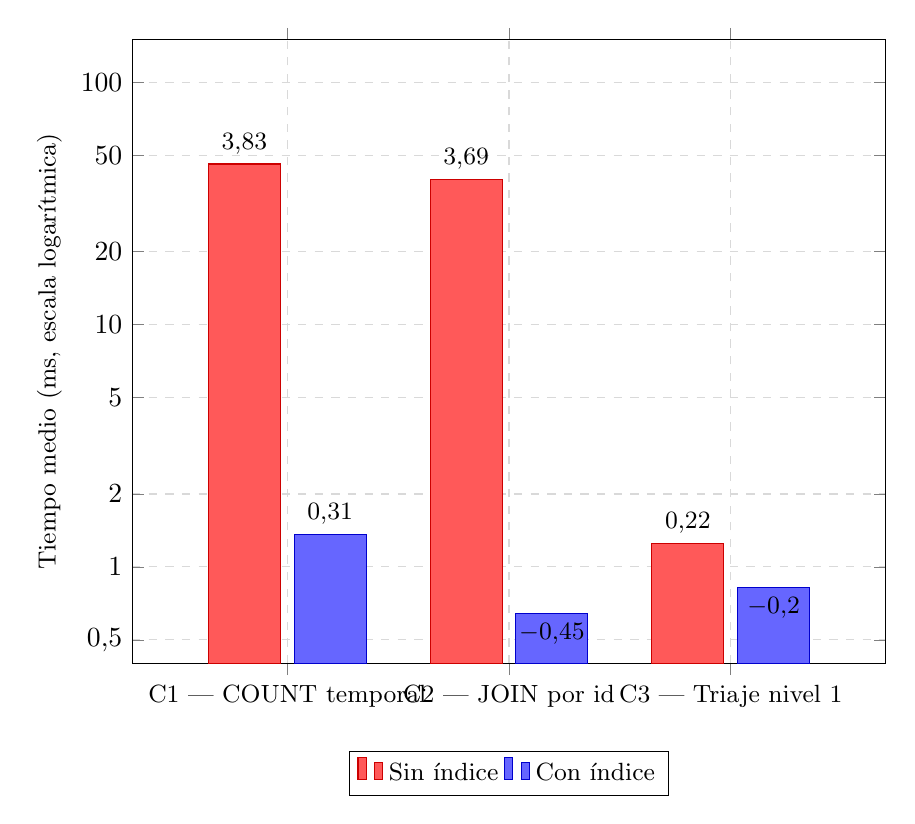
\begin{tikzpicture}
        \begin{axis}[
            ybar=5pt,
            ymode=log,
            log origin=infty,
            bar width=26pt,
            width=0.92\textwidth,
            height=9.5cm,
            ylabel={Tiempo medio (ms, escala logarítmica)},
            ylabel style={font=\small},
            ymin=0.4, ymax=150,
            ytick={0.5,1,2,5,10,20,50,100},
            yticklabels={{0,5}, {1}, {2}, {5}, {10}, {20}, {50}, {100}},
            xtick=data,
            symbolic x coords={C1, C2, C3},
            xticklabels={C1 --- COUNT temporal, C2 --- JOIN por id, C3 --- Triaje nivel 1},
            xticklabel style={font=\small},
            nodes near coords,
            nodes near coords align={vertical},
            every node near coord/.append style={
                font=\small\bfseries, color=black,
                /pgf/number format/.cd, fixed, precision=2, use comma
            },
            legend style={at={(0.5,-0.14)}, anchor=north, legend columns=2, font=\small},
            enlarge x limits=0.35,
            grid=major,
            grid style={dashed, gray!30},
        ]
            \addplot[fill=red!65, draw=red!80!black] coordinates {
                (C1, 46.06)
                (C2, 39.89)
                (C3,  1.25)
            };
            \addlegendentry{Sin índice}

            \addplot[fill=blue!60, draw=blue!80!black] coordinates {
                (C1, 1.36)
                (C2, 0.64)
                (C3, 0.82)
            };
            \addlegendentry{Con índice}
        \end{axis}
    \end{tikzpicture}
    \caption{Impacto de los índices sobre el tiempo de ejecución para las tres consultas (escala logarítmica, media de 50 iteraciones). Cada barra muestra su valor exacto en milisegundos. Los factores de mejora son 33,8×, 62,3× y 1,5× para C1, C2 y C3 respectivamente. C3 ya era rápida sin índice por el reducido tamaño de la tabla MEMORY.}
    \label{fig:grafica_indices}
\end{figure}

\begin{figure}[htbp]
    \centering
    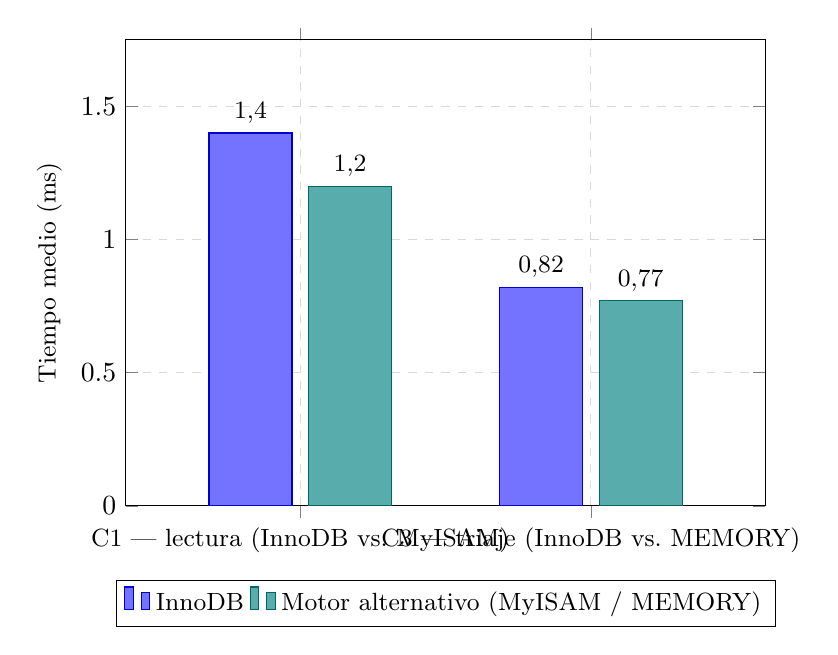
\begin{tikzpicture}
        \begin{axis}[
            ybar=6pt,
            bar width=30pt,
            width=0.8\textwidth,
            height=7.5cm,
            ylabel={Tiempo medio (ms)},
            ylabel style={font=\small},
            ymin=0, ymax=1.75,
            xtick=data,
            symbolic x coords={C1, C3},
            xticklabels={C1 --- lectura (InnoDB vs.\ MyISAM), C3 --- triaje (InnoDB vs.\ MEMORY)},
            xticklabel style={font=\small},
            nodes near coords,
            nodes near coords align={vertical},
            every node near coord/.append style={
                font=\small\bfseries, color=black,
                /pgf/number format/.cd, fixed, precision=2, use comma
            },
            legend style={at={(0.5,-0.16)}, anchor=north, legend columns=2, font=\small},
            enlarge x limits=0.6,
            grid=major,
            grid style={dashed, gray!30},
        ]
            \addplot[fill=blue!55, draw=blue!80!black] coordinates {
                (C1, 1.40)
                (C3, 0.82)
            };
            \addlegendentry{InnoDB}
            \addplot[fill=teal!65, draw=teal!80!black] coordinates {
                (C1, 1.20)
                (C3, 0.77)
            };
            \addlegendentry{Motor alternativo (MyISAM / MEMORY)}
        \end{axis}
    \end{tikzpicture}
    \caption{Comparativa de rendimiento entre motores de almacenamiento con índice activo (media de 50 iteraciones, valor exacto sobre cada barra). En la Consulta~1 (lectura pura) el motor alternativo es MyISAM, que supera a InnoDB por carecer de sobrecarga transaccional; en la Consulta~3 (cola de triaje en tiempo real) el alternativo es MEMORY, que gana a InnoDB al operar íntegramente en RAM.}
    \label{fig:grafica_motores}
\end{figure}

La Tabla~\ref{tab:benchmark_resumen} consolida todos los resultados numéricos.

\begin{table}[htbp]
    \centering
    \caption{Resumen completo de los resultados del benchmarking de consultas (media de 50 iteraciones).}
    \label{tab:benchmark_resumen}
    \small
    \begin{tabular}{llcccp{3.2cm}}
        \toprule
        \textbf{Consulta} & \textbf{Motor} & \textbf{Índice} & \textbf{Tiempo (ms)} & \textbf{Coste est.} & \textbf{Tipo de acceso} \\
        \midrule
        \multirow{3}{*}{C1 — COUNT temporal}
            & InnoDB  & No  & 46,06 & 19.543,10 & Full Table Scan \\
            & InnoDB  & Sí  &  1,36 &    643,62 & Index Range Scan \\
            & MyISAM  & Sí  &  1,20 &        -- & Index Range Scan \\
        \midrule
        \multirow{2}{*}{C2 — JOIN por id}
            & InnoDB  & No  & 39,89 & 17.829,10 & Nested Loop + Full Scan \\
            & InnoDB  & Sí  &  0,64 &        -- & Single Row + Key Lookup \\
        \midrule
        \multirow{3}{*}{C3 — Triaje nivel 1}
            & InnoDB  & No  &  1,25 &     91,82 & Full Table Scan \\
            & InnoDB  & Sí  &  0,82 &     39,65 & Non-Unique Key Lookup \\
            & MEMORY  & Sí  &  0,77 &        -- & Non-Unique Key Lookup \\
        \bottomrule
    \end{tabular}
\end{table}

% ---------------------------------------------------------------------------
\subsubsection{Optimización Espacial: Benchmark de Almacenamiento}
\label{sec:benchmark_espacial}
% ---------------------------------------------------------------------------

El segundo eje de optimización del proyecto es el espacio en disco. La tabla \texttt{historico\_bajas\_medicas} es el caso de uso paradigmático de los datos históricos en un sistema sanitario: se escribe una vez, no se modifica nunca y debe conservarse durante décadas. En España, la normativa obliga a archivar los partes de baja durante al menos cuatro años~\cite{lprl1995}, aunque en la práctica los sistemas de salud los conservan durante periodos mucho mayores. En un sistema que procesa decenas de miles de bajas al año, la eficiencia del almacenamiento de este histórico es un factor de coste relevante.

Para cuantificar el beneficio del motor ARCHIVE sobre InnoDB en este escenario concreto, se crearon dos tablas con estructura idéntica y se insertaron aproximadamente 6.300 registros de bajas médicas en cada una, modificando únicamente la cláusula \texttt{ENGINE} en la definición.

Los resultados obtenidos directamente del \textit{Table Inspector} de MySQL Workbench son concluyentes. La tabla con motor ARCHIVE (Figura~\ref{fig:archive_size}) almacena 6.355 filas en \textbf{533,0 KiB}, con una longitud media de fila de 85 bytes. El campo \textit{Row format} confirma: \texttt{Compressed}.

\begin{figure}[htbp]
    \centering
    
\includegraphics[width=0.58\textwidth]{tamano_en_memoria_con_ARCHIVE.jpg}
    \caption{\textit{Table Inspector} de Workbench para \texttt{historico\_bajas\_medicas} (motor ARCHIVE). 6.355 filas, longitud media de fila 85 bytes, tamaño total 533,0 KiB. Formato de fila: \textit{Compressed}.}
    \label{fig:archive_size}
\end{figure}

La tabla equivalente con motor InnoDB (Figura~\ref{fig:innodb_size}) almacena 6.246 filas —prácticamente el mismo volumen de registros— en \textbf{2,5 MiB} ($\approx$2.560 KiB), con una longitud media de fila de 422 bytes. El campo \textit{Row format} indica: \texttt{Dynamic}.

\begin{figure}[htbp]
    \centering
    
\includegraphics[width=0.58\textwidth]{tamano_en_memoria_con_InnoDB.jpg}
    \caption{\textit{Table Inspector} de Workbench para \texttt{historico\_bajas\_innodb} (motor InnoDB). 6.246 filas, longitud media de fila 422 bytes, tamaño total 2,5 MiB. Formato de fila: \textit{Dynamic}.}
    \label{fig:innodb_size}
\end{figure}

La diferencia es un factor de $4{,}80\times$ a favor de ARCHIVE: InnoDB necesita $2.560$~KiB para almacenar esencialmente los mismos datos que ARCHIVE guarda en $533$~KiB. Expresado como reducción porcentual:

\begin{equation}
    \text{Reducción} = \frac{2560 - 533}{2560} \times 100 = 79{,}2\%
    \label{eq:reduccion}
\end{equation}

La Figura~\ref{fig:grafica_storage} ilustra esta diferencia.

\begin{figure}[htbp]
    \centering
    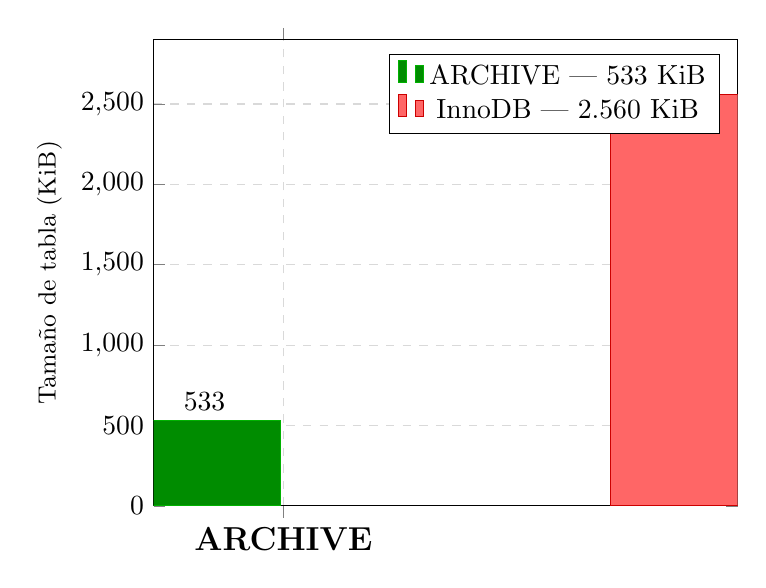
\begin{tikzpicture}
        \begin{axis}[
            ybar,
            bar width=55pt,
            width=9cm,
            height=7.5cm,
            ylabel={Tamaño de tabla (KiB)},
            ylabel style={font=\small},
            ymin=0, ymax=2900,
            xtick=data,
            symbolic x coords={ARCHIVE, InnoDB},
            xticklabel style={font=\large\bfseries},
            nodes near coords,
            nodes near coords align={vertical},
            every node near coord/.append style={font=\normalsize\bfseries},
            enlarge x limits=0.4,
            grid=major,
            grid style={dashed, gray!30},
            legend style={at={(0.97,0.97)}, anchor=north east},
        ]
            \addplot[fill=green!55!black, draw=green!70!black]
                coordinates {(ARCHIVE, 533)};
            \addlegendentry{ARCHIVE — 533 KiB}
            \addplot[fill=red!60, draw=red!80!black]
                coordinates {(InnoDB, 2560)};
            \addlegendentry{InnoDB — 2.560 KiB}
        \end{axis}
    \end{tikzpicture}
    \caption{Comparativa de espacio en disco entre los motores ARCHIVE e InnoDB para $\approx$6.300 registros de bajas médicas. ARCHIVE almacena los mismos datos ocupando un 79,2\% menos de espacio gracias a la compresión \textit{zlib} fila a fila.}
    \label{fig:grafica_storage}
\end{figure}

La clave de la diferencia está en la longitud media de fila: 85 bytes por registro en ARCHIVE frente a 422 bytes en InnoDB, un ratio de $4{,}97\times$. InnoDB almacena cada fila en formato \texttt{Dynamic} con la extensión original de todos los campos más la cabecera del registro, los punteros de versión del MVCC y el espacio necesario para el \textit{undo log}. El motor ARCHIVE, al renunciar por completo a las capacidades transaccionales, puede aplicar compresión \textit{zlib} en el momento de la inserción y eliminar toda la infraestructura de gestión transaccional, reduciendo el tamaño de cada fila a lo estrictamente necesario para almacenar el dato.

Para poner en perspectiva el impacto a escala real: un sistema de salud regional que gestione 200.000 bajas médicas al año acumularía, en un periodo de diez años, dos millones de registros. Con InnoDB, ese volumen ocuparía aproximadamente $\frac{2\,000\,000}{6\,300} \times 2.560\,\text{KiB} \approx 813\,\text{GB}$. Con ARCHIVE, la cifra se reduciría a unos $170\,\text{GB}$: un ahorro de más de $640\,\text{GB}$ en almacenamiento primario, con el consiguiente impacto en costes de infraestructura, tiempos de backup y velocidad de los procesos de archivado y recuperación.

\end{document}
